\documentclass[DM,authoryear,toc]{lsstdoc}
% lsstdoc documentation: https://lsst-texmf.lsst.io/lsstdoc.html
\input{meta}

% Package imports go here.

% Local commands go here.

%If you want glossaries
%\input{aglossary.tex}
%\makeglossaries

\title{DM Calibration Products}

% Optional subtitle
% \setDocSubtitle{A subtitle}

\author{%
Christopher Z Waters
}

\setDocRef{DMTN-148}
\setDocUpstreamLocation{\url{https://github.com/lsst-dm/dmtn-148}}

\date{\vcsDate}

% Optional: name of the document's curator
% \setDocCurator{The Curator of this Document}

\setDocAbstract{%
The goal of this tech note is to provide a plan for the handling of calibration products in the Gen-3 Butler environment, including the construction, validation, certification, and deprecation.  This process is equally challenging with the current Gen-2 Butlers, but the hope is that with a clear goal in mind, the currently existing calibrations, for all calibration types and cameras, can be migrated to a common design that will be shared with Gen-3.  The current state, the end goal, and the transition steps between these are defined.
}

% Change history defined here.
% Order: oldest first.
% Fields: VERSION, DATE, DESCRIPTION, OWNER NAME.
% See LPM-51 for version number policy.
\setDocChangeRecord{%
  \addtohist{1}{2020-04-16}{Initial version.}{Christopher Waters}
  \addtohist{2}{2020-12-31}{Updates to represent how calibrations were actually made.}{Christopher Waters}
}


\begin{document}

% Create the title page.
\maketitle
% Frequently for a technote we do not want a title page  uncomment this to remove the title page and changelog.
% use \mkshorttitle to remove the extra pages

% ADD CONTENT HERE
% You can also use the \input command to include several content files.

\section{Intro}

The goal of this tech note is to provide a plan for the handling of
calibration products in the Gen-3 Butler environment.  There are a
large number of these products currently in use, but many of them do
not have a clearly defined process to define, ingest, test, and
deprecate them.  The lack of documentation on how these processes work
has led to many implementations of similar paths, further complicating
the issue.


\section{The End State}

The final state that we wish to get to has the following properties:

\begin{itemize}
\item All calibration products are either lsst.afw.image.Exposure
  image data or a subclass of the \verb|CalibType| calibration class
  from the \verb|ip_isr| package.
%% CZW: input data => raw images.
%%      single vs multiple pipelines.
%%      provenance as a butler exportable object.
\item As much as possible, all calibration products should be
  constructed by a DM Task in the \verb|cp_pipe| package.  The raw
  input data used for the construction will be available from the
  Gen-3 Butler, and can be exported along with the task configuration
  parameters to allow these calibrations to be reconstructed in the
  future.  Exceptions will exist for external or lab created
  calibrations, although we expect the number of these calibrations to
  be small.
\item The provenance, config, and final product files may be saved to
  an \verb|obs_CAMERA_data| package in git for convenience.  This
  allows these files to be directly migrated to other Butler
  repositories without being reconstructed.  Making these products
  human readable allows the tracking of value changes with the
  evolution of the set of exported products.
%% CZW: Prior calibrations used for live raw data.
%%      cp_verify to show that live calibrations are consistent with that.
\item All calibration products will be verified prior to
  certification.  The goal of this process is to demonstrate that the
  newly constructed calibration satisfies a number of quantifiable
  quality checks.  This should reduce the amount of manual image
  examination necessary for certification.  DMTN-101 will define the
  exact tests for each calibration type.
\item All calibration products are certified for use and have the
  valid date range set manually, preventing test runs from being used
  inadvertently.  Calibrations ingested from an \verb|obs_CAMERA_data|
  package in git should have sufficient metadata that supply
  appropriate date ranges.
\item The verification pipeline will also be run on new raw
  calibration data.  This will ensure that the certified calibrations
  being used for the live raw data stream are appropriate, and to
  monitor the variations of the defined metrics with time.
\item Calibration information stored in a lsst.afw.cameraGeom object
  may be used, but is always assumed to be overridden by supplied
  calibration products.  No new calibration information should be
  stored in these objects, and currently existing calibration
  information should be deprecated.

\end{itemize}

\section{The Current State}

\subsection{Standard Calibrations}


%% CZW: collection namning consistent with RFC-741/DMTN-167
The classic calibration products, \verb|BIAS|, \verb|DARK|,
\verb|FLAT|, and \verb|FRINGE|, all write FITS files that are indexed
in Butler's calibRegistry.sqlite3 repository database.  These files
are created by \verb|pipe_drivers|/constructCalibs.py, and are
ingested into the repository upon acceptance by
\verb|pipe_tasks|/ingestCalibs.py.  This ingestion process sets the
``validStart'' and ``validEnd'' values to restrict the usage of the
calibration, as well as some identifying string which is used (along
with calibration type, filter, and detector) to uniquely identify the
calibration on disk.  We have been using the ``calibDate'', indicating
when the calibration was constructed or ingested, as this string.  For
calibrations that are generated by \verb|cp_pipe|, it may be better to
use the Butler collection that the calibration was generated in (which
will enforce uniqueness on simultaneous processing).  Calibrations
that are ingested from git could use the repository SHA1 hash, which
would provide similar uniqueness.

Although not formally a ``classic'' calibration product, the \verb|SKY|
calibration is produced, stored, and accessed the same way.

\subsection{``User-curated'' Calibrations}

The other inputs necessary for ISR have generally been described as
"user-curated".  These products are either defined by the \verb|CAMERA| as
part of the afw.cameraGeom description of the instrument, or are
variously persisted and accessed in unique ways.  Describing a path to
fixing this is a goal of this tech note.

As part of the \verb|DEFECTS| rework (RFC-595), there is now a fixed and
generic way to handle the ingest, if not necessarily the construction,
of that product.  The \verb|QE_CURVE| (RFC-625) has been implemented
following this process.  These \verb|DEFECTS|-like calibration products have
their origins as human-curated text files in the appropriate
\verb|obs_CAMERA_data| packages (and are thereby versioned through the
packages' git repositories).  The text file must be in a structured
format, to allow the header keywords to be read and assigned to a
metadata PropertyList.

For these products to be used, they must be converted into a FITS
format that can be read by ingestCalibs.py.  This is performed by the
\verb|pipe_tasks|/ingestCuratedCalibs.py script, which uses the metadata
information and the calibration product's python class to read the
text version and convert to a FITS file format that can be ingested by
ingestCalibs.py.

This updated calibration process removes the necessity that each
\verb|obs_CAMERA_data| package implement one-off mapper methods to allow the
product to be found.  However, only \verb|DEFECTS|, \verb|QE_CURVE|, and \verb|LINEARITY|
follow this system, leaving the remaining products to be handled with
camera-specific code and cameraGeom entries.  In addition to having
diverse implementations, these handlers are often rigid, and cannot be
versioned easily.

\section{Transitioning to Gen3/What We Should Expect From Gen3}

\subsection{Figures}

\begin{figure}
  \caption{Standard calibration creation.}
  \centering
  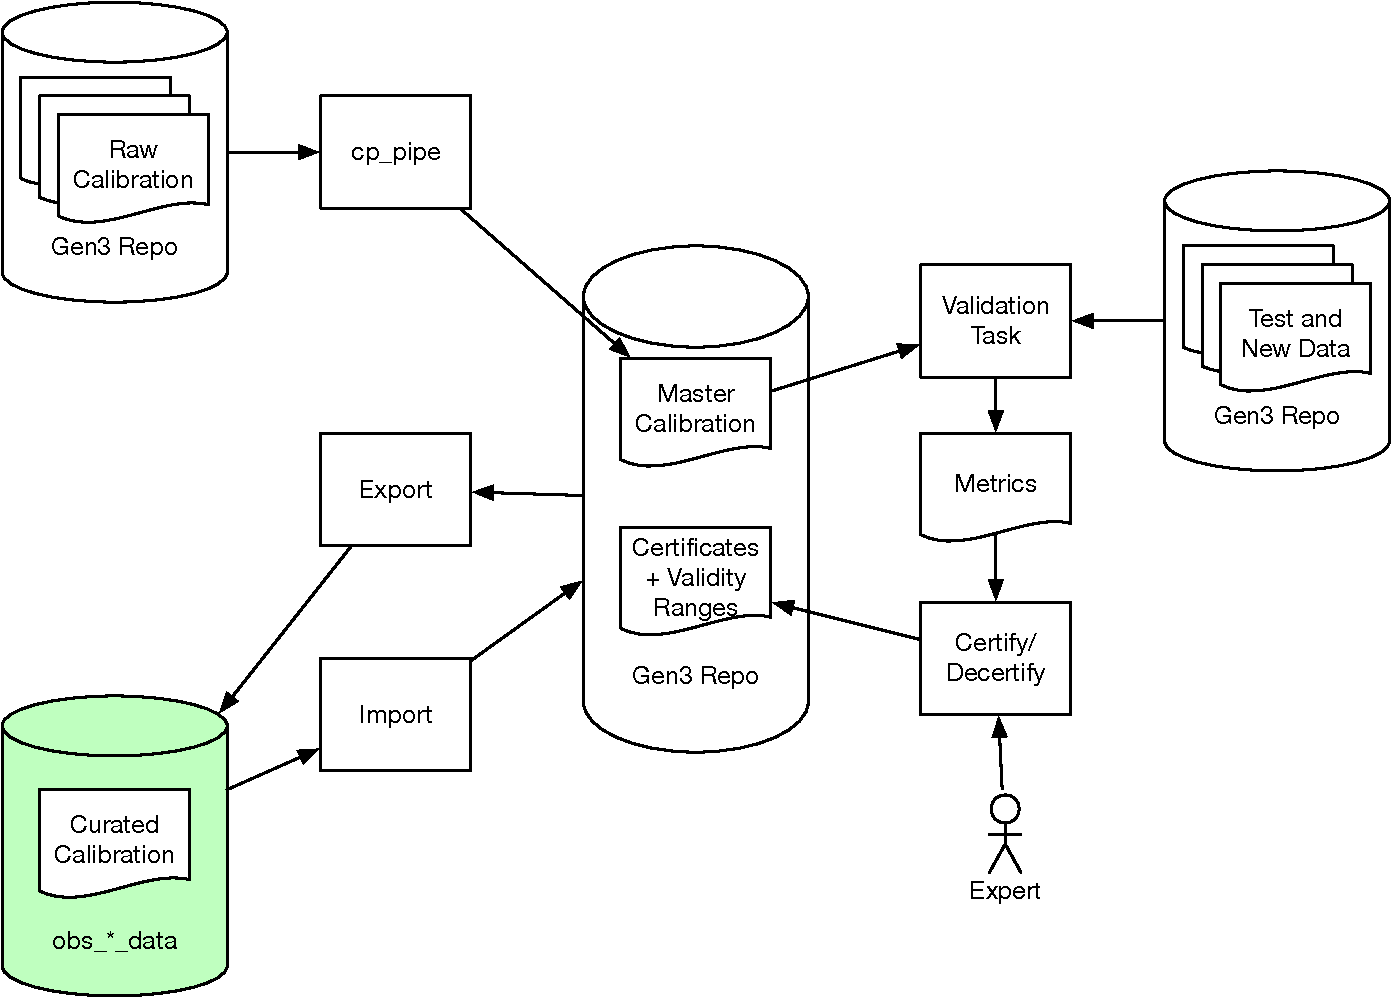
\includegraphics[width=0.9\textwidth]{figures/Standard_Calibration.pdf}
\end{figure}

\begin{figure}
  \caption{Hand-Edited calibration creation.}
  \centering
  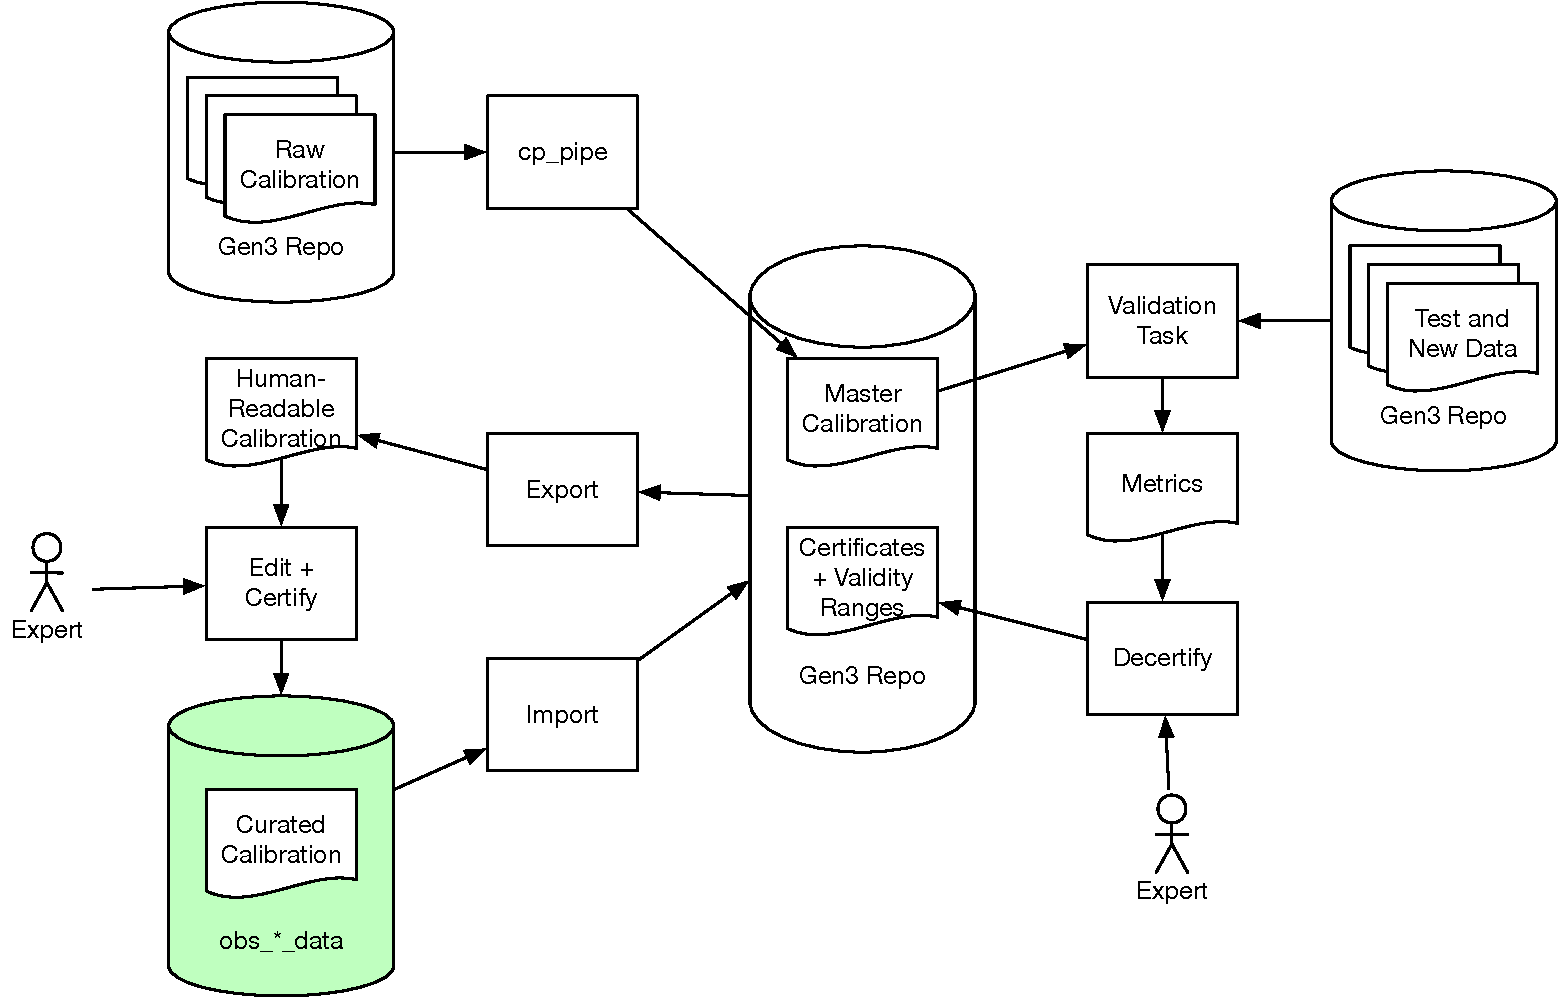
\includegraphics[width=0.9\textwidth]{figures/Hand-Edited_Calibration.pdf}
\end{figure}

\begin{figure}
  \caption{External calibration ingest.}
  \centering
  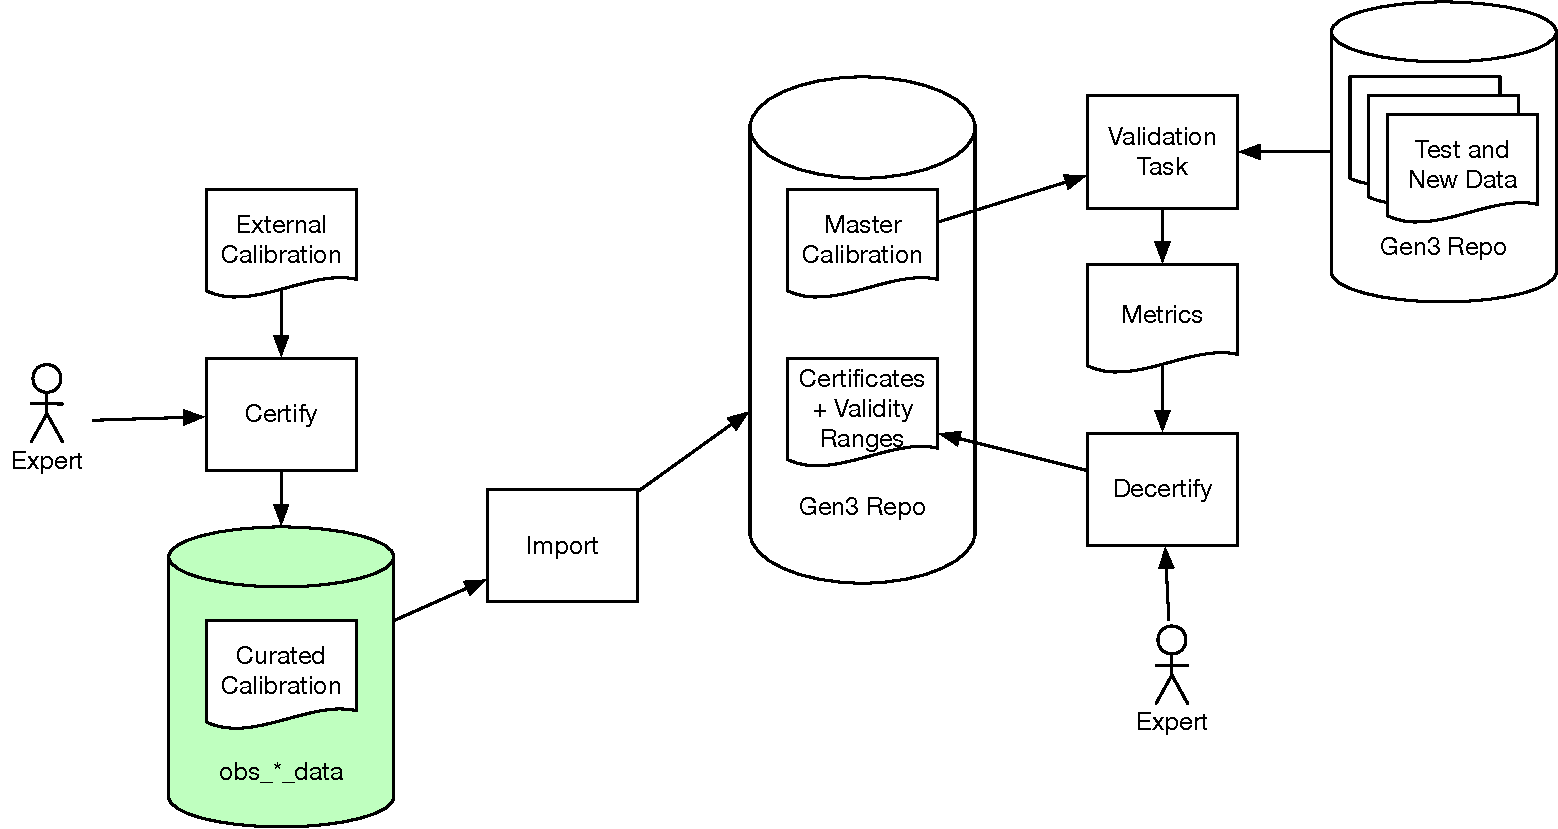
\includegraphics[width=0.9\textwidth]{figures/External_Calibration.pdf}
\end{figure}


\subsection{A CalibrationBaseClass}
The first step to a consistent calibration system is to ensure that
all products in both generations use the \verb|DEFECTS|-like calibration
product system.  For FITS image products, this requires future
calibrations to be constructed with all of the header keyword values
listed below.

%% CZW: discuss file format.
%%      FITS as the default format, existing formatter.
The remaining unconverted calibration types (\verb|CROSSTALK|, \verb|BFKERNEL|)
should be converted to use \verb|DEFECTS|-like class, most likely by defining
a CalibrationBaseClass, and making all of the calibration products
subclasses of that.  This would enforce that all calibrations can be
relied upon to provide getMetadata, setMetadata, readFits, writeFits,
readText, and writeText methods.  Gen2 Butler instances would then be
able to access all calibration products in a single consistent manner.
This also ensures that Gen2 and Gen3 can use the same calibration
products.

\subsection{Metadata and Header Keywords}

The required header keywords are currently poorly standarized.  The
\verb|OBSTYPE| keyword is universally populated in all calibrations,
regardless of if they are generated by constructCalibs.py or are
curated by the \verb|obs_CAMERA| packages.  Curated calibrations also
require the \verb|DETECTOR| and \verb|CALIBDATE|, the last of which is
also populated by constructCalibs.py.  The \verb|CALIB_ID| is set by
constructCalibs.py, and exists for the majority of curated
calibrations, but is not consistently used.

The keywords listed in table \ref{tab:metadata} are the proposed list
of header keywords that will be required in the new operational
calibrations in Gen3.  The majority of these are inserted at creation,
identifying the content and applicable data range for the calibration.
Only upon certification (the replacement for the Gen2 ingest) are the
valid date ranges set.  To conform with the expected changes to FITS
persistence in RFC-686, these and all other calibration-specific
metadata fields will be upper-case.

\begin{tabular}{l l l}
  \label{tab:metadata}
  Keyword & Inserted & Description \\
  \hline
  %% CZW: SCHEMA and VERSION duplicate each other.
  \verb|OBSTYPE| & Creation & Calibration dataset type contained in this file. \\
  \verb|{OBSTYPE}_SCHEMA| & Creation & Storage schema for calibration.  \\
  \verb|{OBSTYPE}_VERSION| & Creation & Storage schema version. \\
  \verb|INSTRUME| & Creation & Instrument/camera this calibration belongs to. \\
  \verb|DETECTOR| & Creation & Integer identifier for the ccd/detector. \\
  \verb|FILTER| & Creation & Name of the physical filter or ``NONE''. \\
  \verb|CALIB_ID| & Creation & DataId that can be used to request this calibration after ingest. \\
  \verb|CALIB_CREATION_DATE| & Creation & Creation date of the calibration. \\
  \verb|CALIB_CREATION_TIME| & Creation & Creation time of the calibration. \\
  \verb|CALIBDATE| & Creation & Concatenation of \verb|CALIB_CREATION_DATE| and \verb|CALIB_CREATION_TIME|. \\
  \verb|VALIDSTART| & Certification & Start date the calibration is valid from.  \\
  \verb|VALIDEND| & Certification & End date the calibration is valid from.  \\
\end{tabular}

\begin{tabular}{l l}
  Keyword & Description \\
  \hline
  %% CZW: detector is an integer.
  %%      calib_id contents
  %%      split creation date/time still necessary?
  %%      validity range is a butler option.
  \multicolumn{2}{c}{Keywords available as calibration properties.}
  \verb|OBSTYPE | & Calibration dataset type contained in this file. \\
  \verb|{OBSTYPE}_VERSION| & Storage schema version, to allow backwards compatibility. \\
  \verb|INSTRUME| & Instrument/camera this calibration belongs to. \\
  \verb|RAFTNAME| & Raft containing the detector. \\
  \verb|SLOTNAME| & Slot in the raft containing the detector. \\
  \verb|DETECTOR| & Integer identifier for the ccd/detector. \\
  \verb|DET_NAME| & String identifier for the detector. \\
  \verb|DET_SER | & Serial number string uniquely identifying the detector device. \\
  \verb|FILTER  | & Name of the physical filter or ``NONE''. \\
  \verb|CALIB_ID| & String containing the dataId that is used during ingest. \\
  \hline
  \multicolumn{2}{c}{Keywords set at creation time.}
  \verb|CALIB_CREATION_DATE| & Creation date of the calibration. \\
  \verb|CALIB_CREATION_TIME| & Creation time of the calibration. \\
  \hline
  \multicolumn{2}{c}{Keywords that are set on export from Butler.}
  \verb|CALIBDATE| & As used, is the validity start date for the calibration. \\
  \verb|VALIDSTART| & The start date of the validity range for the calibration. \\
  \verb|VALIDEND| & The end date of the validity range for the calibration. \\
\end{tabular}


\subsection{Calibration Construction in Gen3}

Calibration products should be constructed using well defined
PipelineTask code.  This removes the need to delineate between
``calibrations'' and ``user-curated calibrations''.  The only
remaining difference between these two groups is what the initial
persisted data type is: ``calibrations'' are stored in FITS images, as
they represent corrections that are only meaningful as full images;
``user-curated calibrations'' can be visualized in a small number of
parameters, and so persisting these in a text format to allow user
inspection is reasonable.  ECSV and YAML are good formats for these
calibrations, and a calibration's readText/writeText methods should
implement one of these.

%% CZW: duplicate provenance.
In addition to the calibration product, the PipelineTask code must
persist a record of the input data used for construction.  This, along
with the already persisted pipeline definition and task configuration,
allows the calibration to be regenerated by any user, making the
construction process much more transparent than it currently is.  A
YAML file containing the dataId parameters for all inputs would
satisfy this.  Appending additional construction statistics (for
example, weight factors applied to each input during the combination
stage) would be helpful in the validation process.

% CZW: Define OIDF = CALIB_ID
Newly generated calibration products will belong to a Gen3 collection,
and that collection will be used to manage the calibration through the
validation and certification process.  This collection may only
contain one entry for a given OIDF set.

\subsection{Validation}

% CZW: Point to DMTN-101 update
%      Define ``new data''
%      input validation, held back validation, new data validation
%      Metrics TBD/DMTN-101
Calibration products are not currently validated, largely due to the
opaque construction process.  Some set of proper validation tasks must
be made, applying the newly constructed product to a set of test
exposures prior to that calibration product's certification.  Applying
these validation tasks continuously as new data is taken will inform
the date ranges for which the product is certified.

\subsection{Certification}

% CZW: File format cannot change on registration.
%      Handling validation ranges.
%      Header update on export?
%      Source of truth => gen3.  obs_camera_data => exportability.
Once a calibration product has been confirmed through validation to
correct the instrument effect it is designed for, it will be certified
with a date range denoting when the calibration is valid, and assigned
to a particular calibration collection (which may contain calibrations
the same OIDF values, as the validity range adds another dimension).
For FITS image calibrations, this is equivalent to a database
operation; no persisted data need change.  This is also acceptable for
text calibrations, although conversion to FITS (using the
CalibrationBaseClass methods) may be desired for IO speed. In
addition, as the text calibrations are human readable and easier to
manage, they should be exported to the appropriate \verb|obs_CAMERA_data|
package.  This provides a common versioned repository for the state of
the camera calibration that can be exported and used independently of
the Gen3 repository where they were constructed.  These exports should
also include the configuration and input data records.

\subsection{Modifying Calibrations}

Most calibration products need user intervention only to launch the
construction and to validate and certify the result.  However, it is
assumed that some of the products used (such as \verb|CAMERA| and
\verb|QE_CURVE| definitions) will not have a PipelineTask construction
process.  The version of these products stored in the
\verb|obs_CAMERA_data| (or \verb|obs_CAMERA| for the case of the
\verb|CAMERA| calibration) repository will be ingested into the Butler
repository as needed.  These products should still have as much
configuration and provenance data as is possible, but should also note
any manual edits with a name and date.  Enforcing the inclusion of the
\verb|obs_CAMERA_data| packages git repository SHA1 entry into the
metadata of calibration products that have been ingested from those
packages should provide sufficient information to reproduce or revert
the manual edits.  This provenance method should also be used for
calibrations that need to be augmented in non-algorithmic ways, such
as \verb|DEFECTS|.

\subsection{Deprecating Calibrations}

Calibrations that should no longer be used (due to code improvements
or newly discovered problems) can be deprecated in Gen3 with
operations on the calibration collection that contains them.  This
will require tools for collection management, but this will be
entirely Butler database operations and will likely not be calibration
specific.


\section{Conclusion}



\appendix
% Include all the relevant bib files.
% https://lsst-texmf.lsst.io/lsstdoc.html#bibliographies

\begin{tabular}{l |c|c|l|l}
  Calibration product & Gen-2 Form & Gen-3 Form & Notes \\
  \hline
  \verb|BIAS| & & & \\
  \verb|DARK| & & & \\
  \verb|FLAT| & & & \\
  \verb|FRINGE| & & & \\
  \verb|SKY| & & & \\
  \verb|CAMERA| & & & \\
  \verb|DEFECTS| & & & \\
  \verb|CROSSTALK| & & & \\
  \verb|LINEARITY| & & & \\
  \verb|BFKERNEL| & & & \\
  \verb|QE_CURVE| & & & \\
  \verb|STRAYLIGHT| & & & \\
  \verb|ILLUMINATION| & & & \\
\end{tabular}

\section{References} \label{sec:bib}
\bibliography{local,lsst,lsst-dm,refs_ads,refs,books}

% Make sure lsst-texmf/bin/generateAcronyms.py is in your path
\section{Acronyms} \label{sec:acronyms}
\addtocounter{table}{-1}
\begin{longtable}{p{0.145\textwidth}p{0.8\textwidth}}\hline
\textbf{Acronym} & \textbf{Description}  \\\hline

DM & Data Management \\\hline
DMTN & DM Technical Note \\\hline
FITS & Flexible Image Transport System \\\hline
ISR & Instrument Signal Removal \\\hline
OIDF & The set of (\verb|OBSTYPE|, \verb|INSTRUME|, \verb|DETECTOR|, \verb|FILTER|). \\\hline
RFC & Request For Comment \\\hline
YAML & Yet Another Markup Language \\\hline
\end{longtable}

% If you want glossary uncomment below -- comment out the two lines above
%\printglossaries





\end{document}
